\documentclass{article}
\usepackage{graphicx} %package to manage images
\usepackage[utf8]{inputenc}
\usepackage[a4paper, total={6in, 8in}]{geometry}
\usepackage{xurl}
\usepackage{hyperref}
\usepackage{float}
\title{Relatório 10 \\ ROC curves}
\author{Pedro A. S. O. Neto}
\date{Setembro, 2023}

\begin{document}

\maketitle

\section{ROC curves - Versão 2}

\begin{figure}[H]
  \caption{Matched proportions}
  \noindent\makebox[\textwidth]{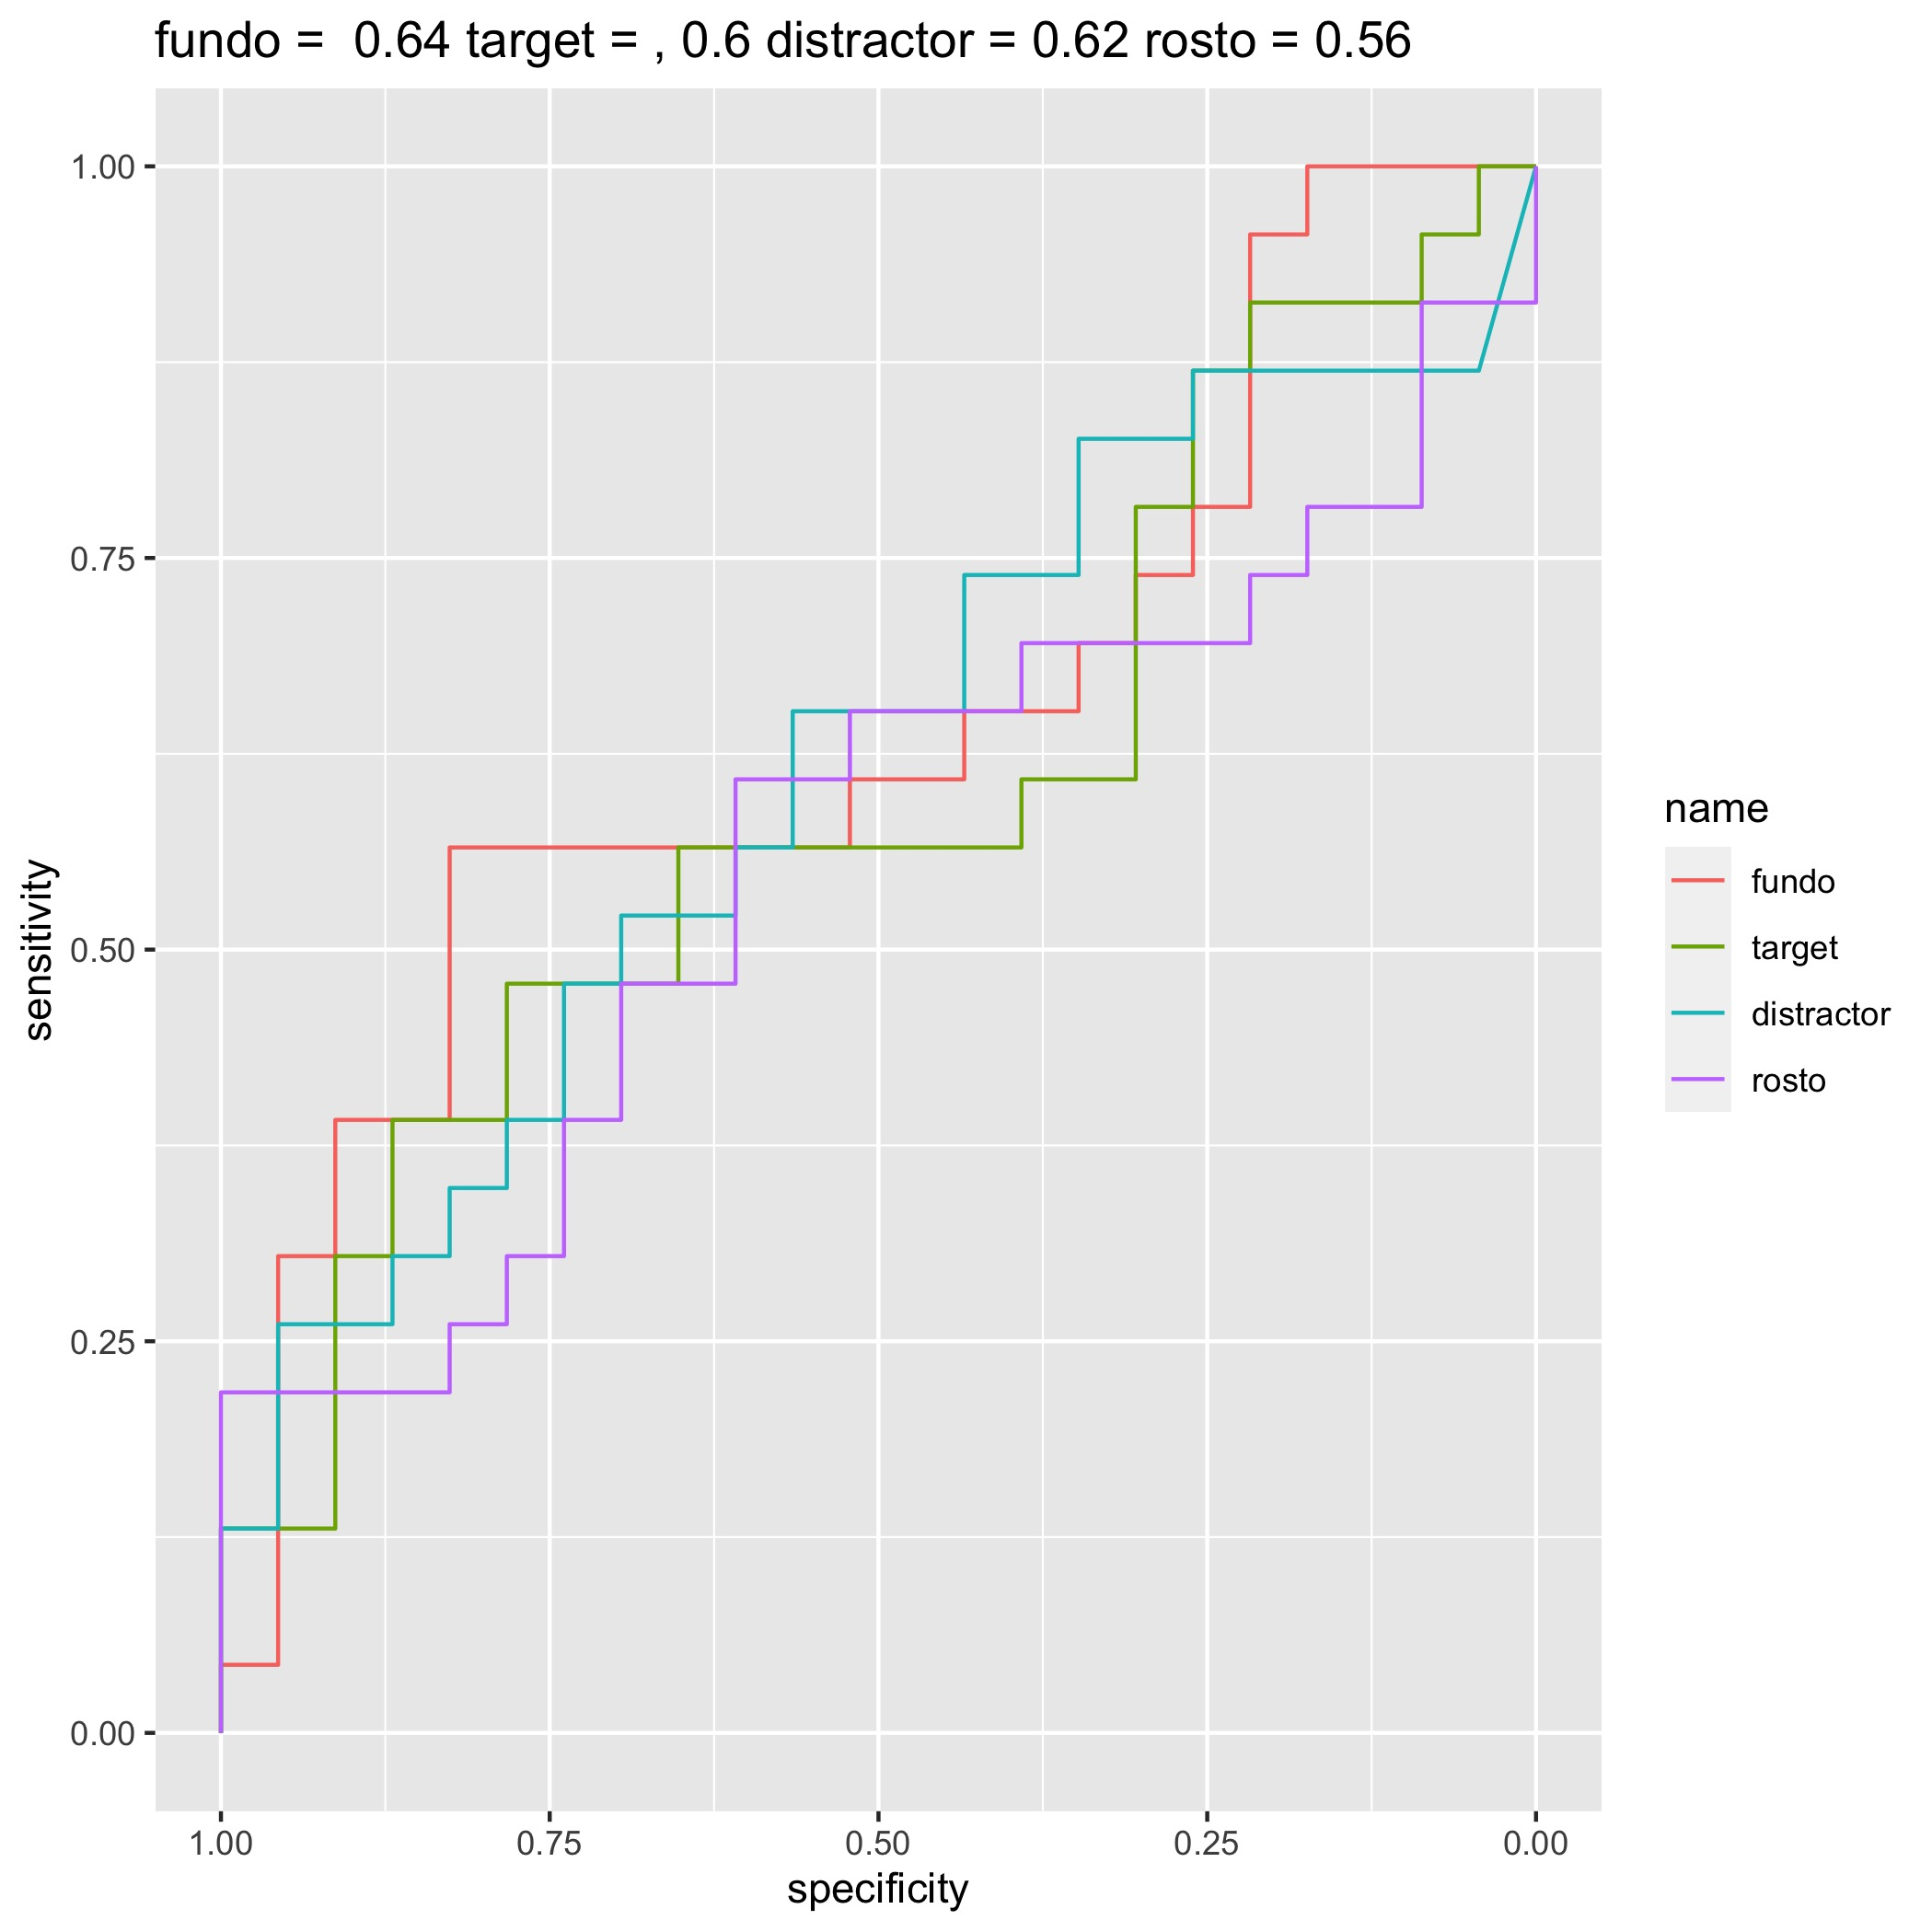
\includegraphics[scale=0.2]{./proportionMatched.jpg}}
  \centering
\end{figure}

\begin{figure}[H]
  \caption{Non matched proportions}
  \noindent\makebox[\textwidth]{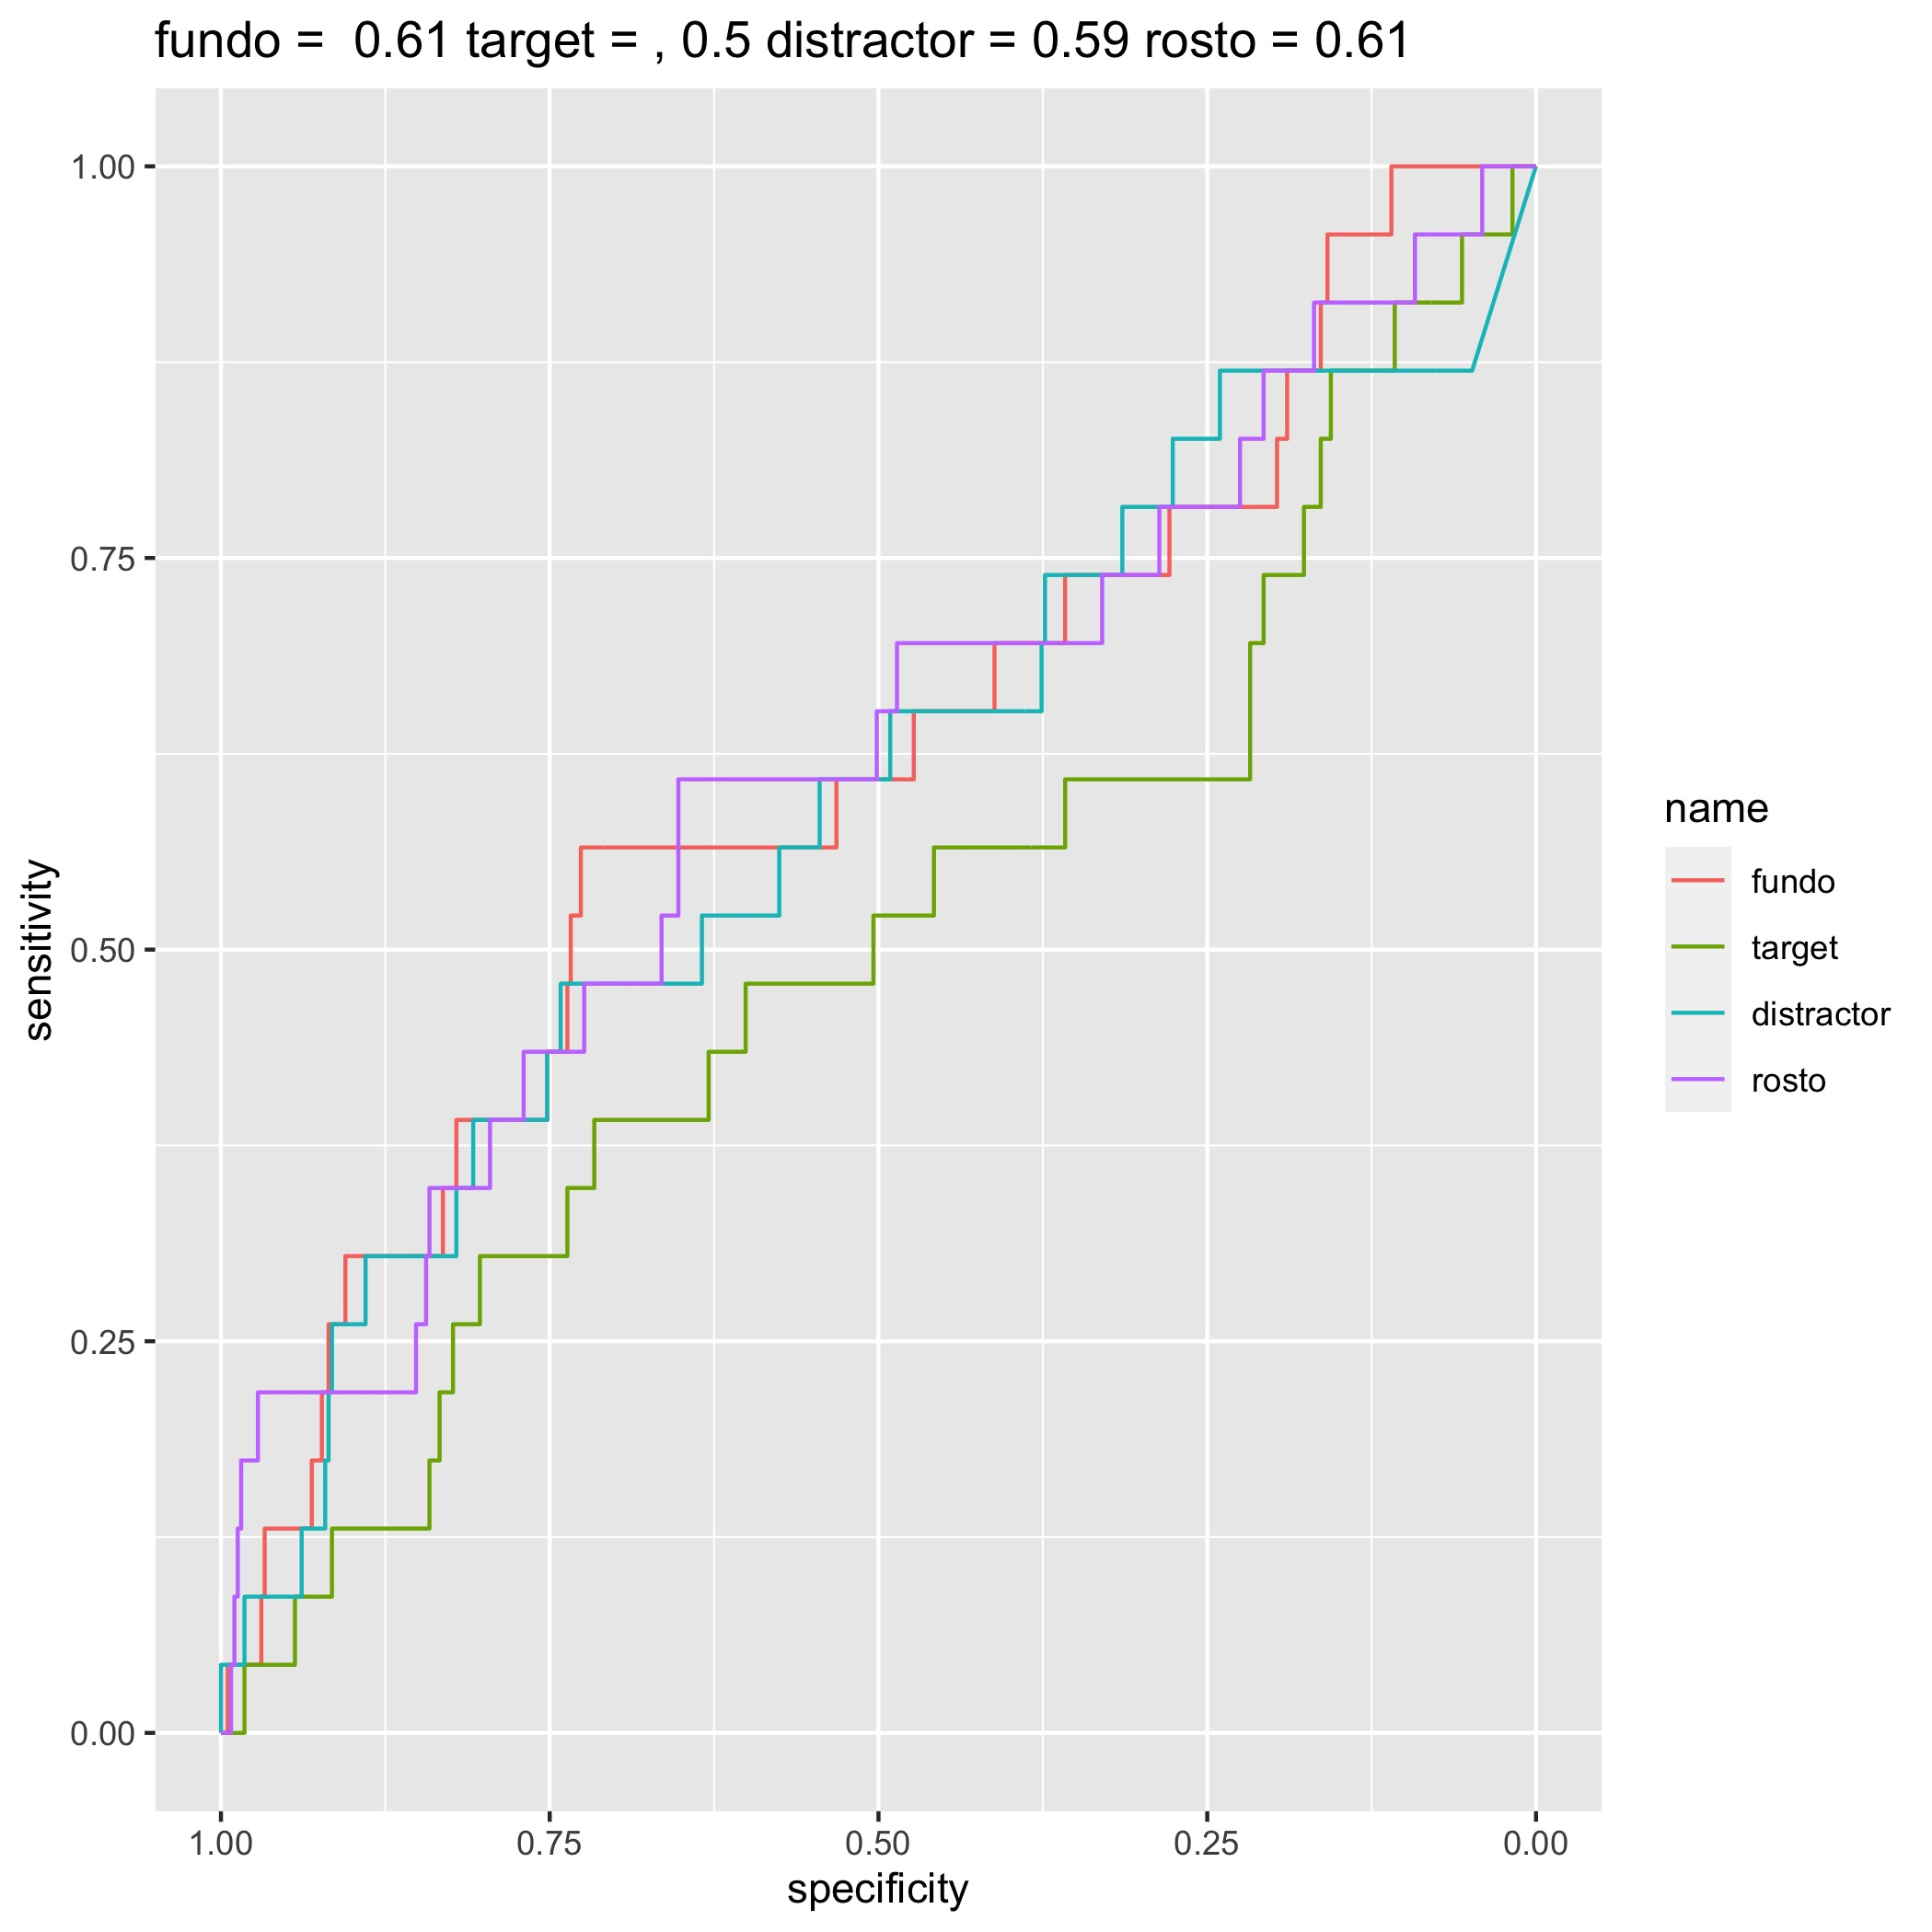
\includegraphics[scale=0.2]{./proportionNonMatched.jpg}}
  \centering
\end{figure}

\begin{figure}[H]
  \caption{Alternancia matched}
  \noindent\makebox[\textwidth]{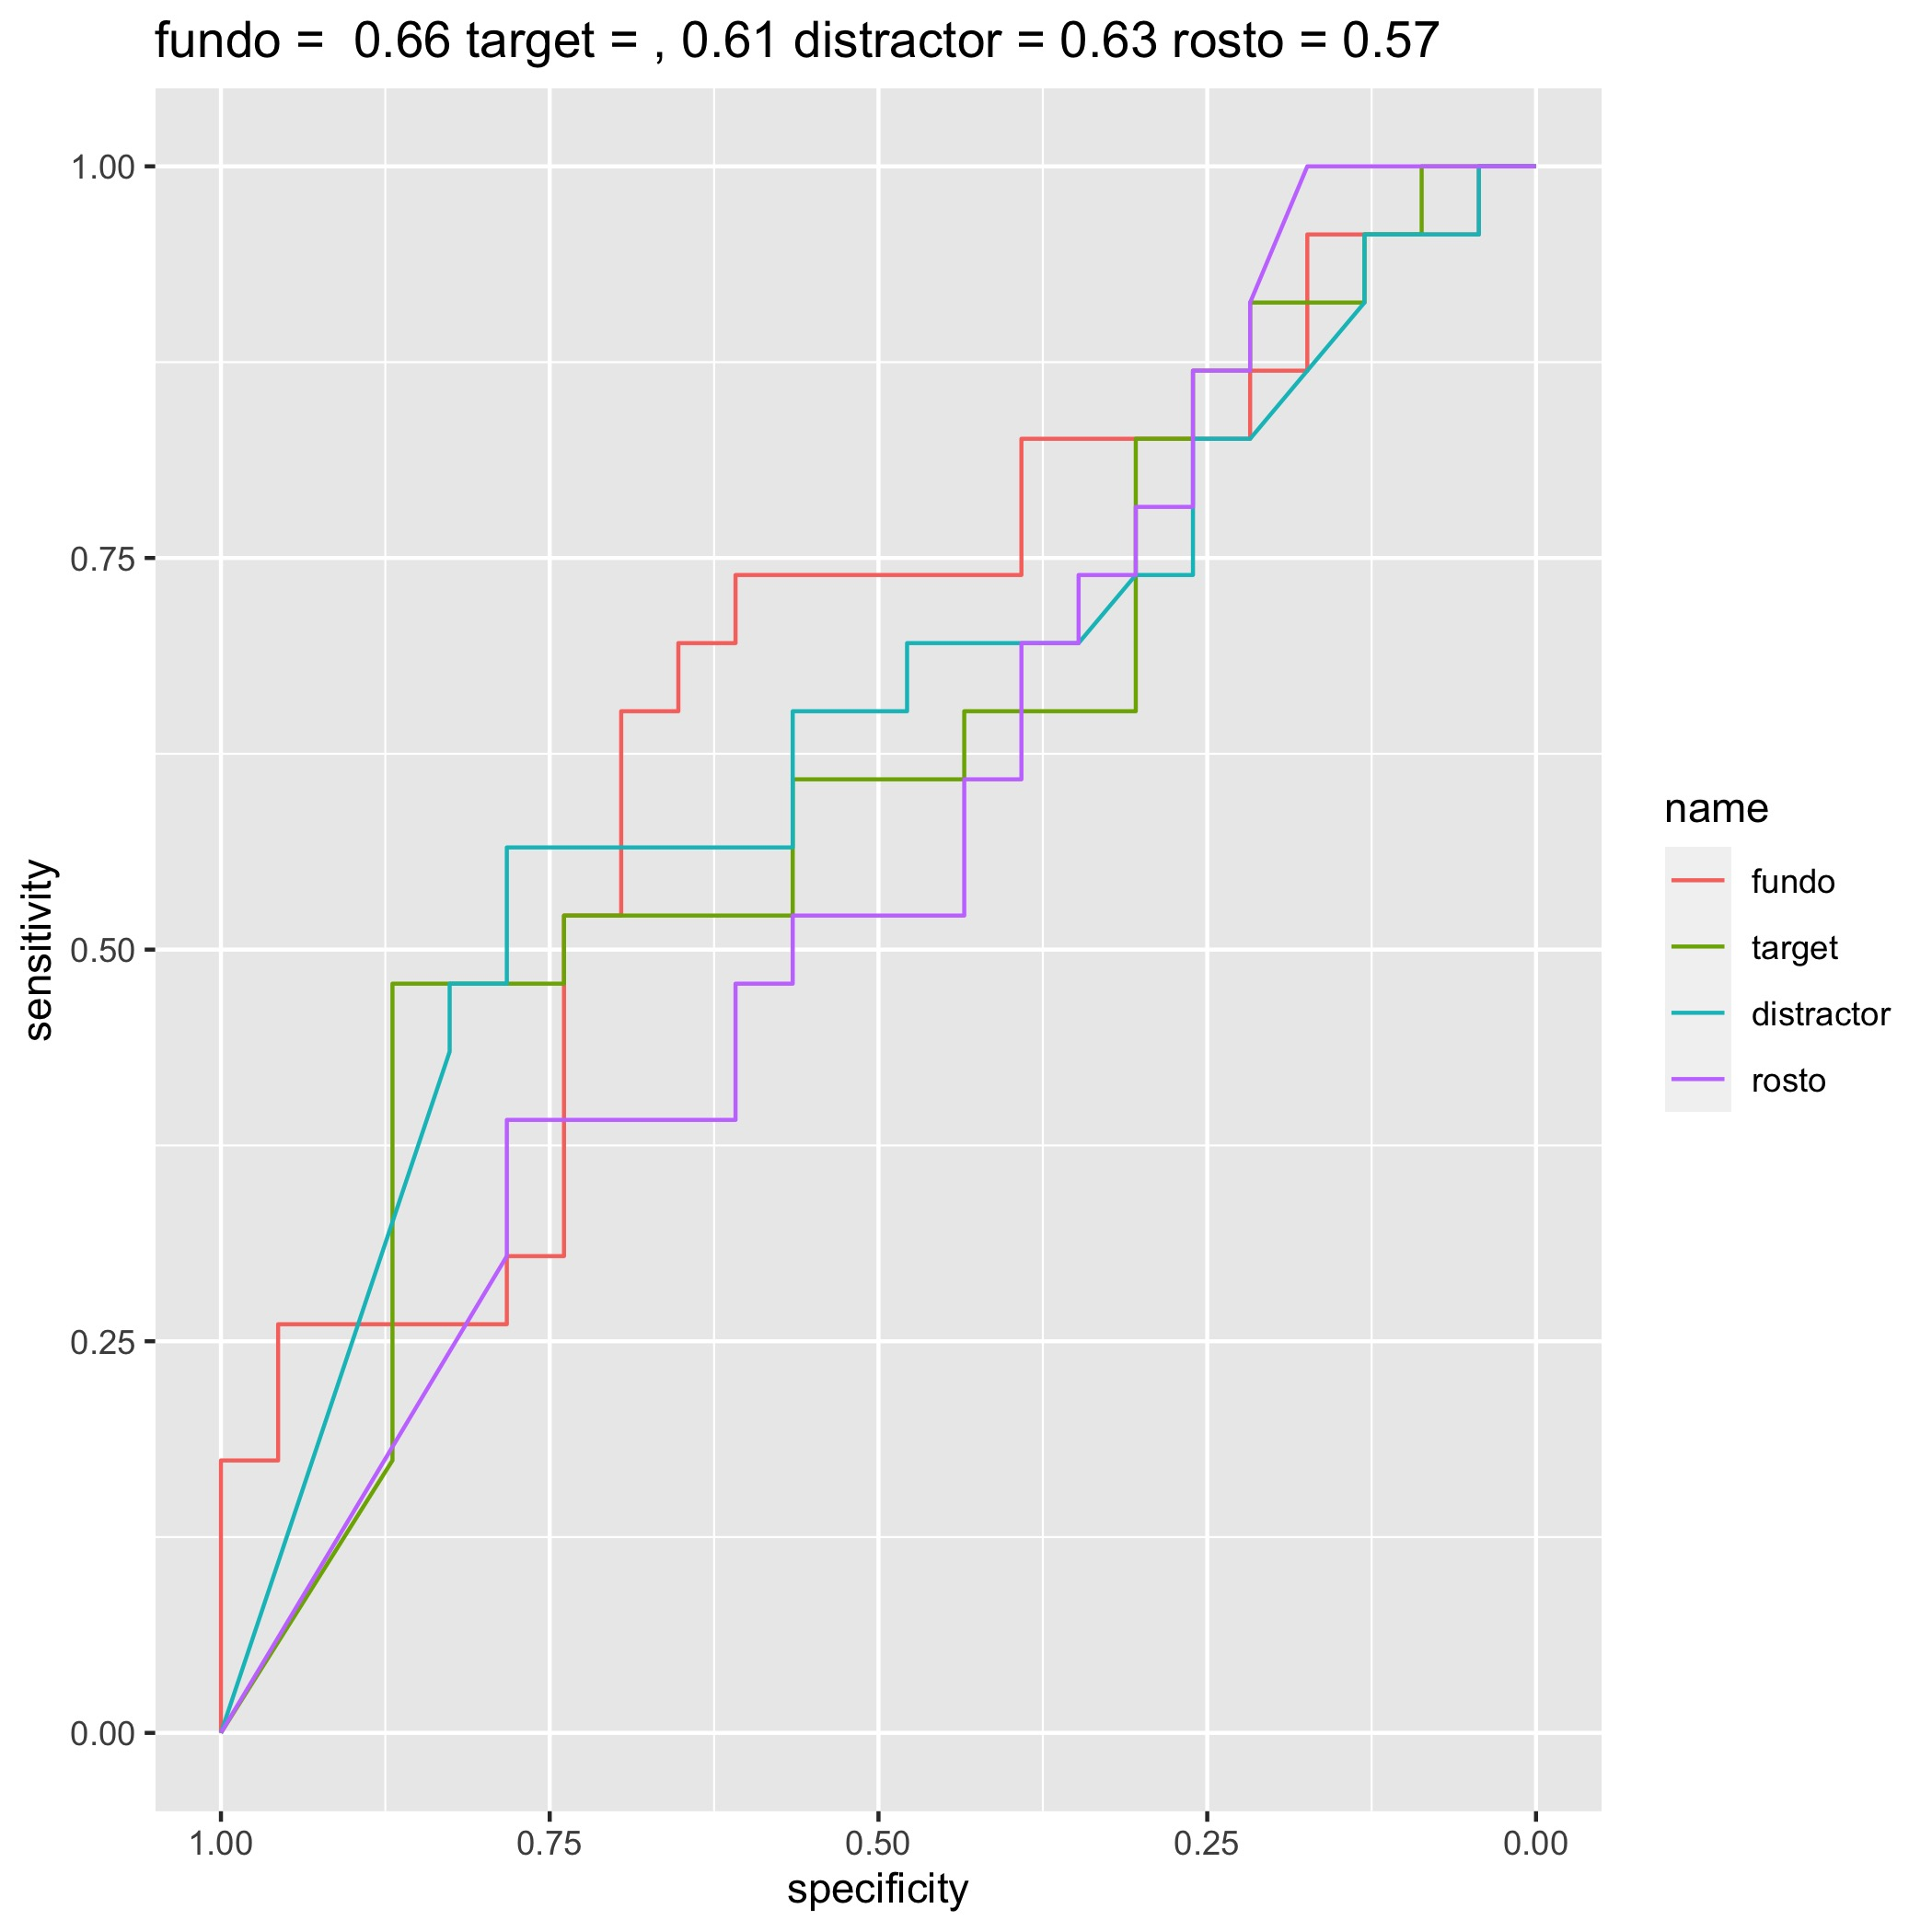
\includegraphics[scale=0.2]{./alternanciaMatched.jpg}}
  \centering
\end{figure}

\begin{figure}[H]
  \caption{Non matched alternancia}
  \noindent\makebox[\textwidth]{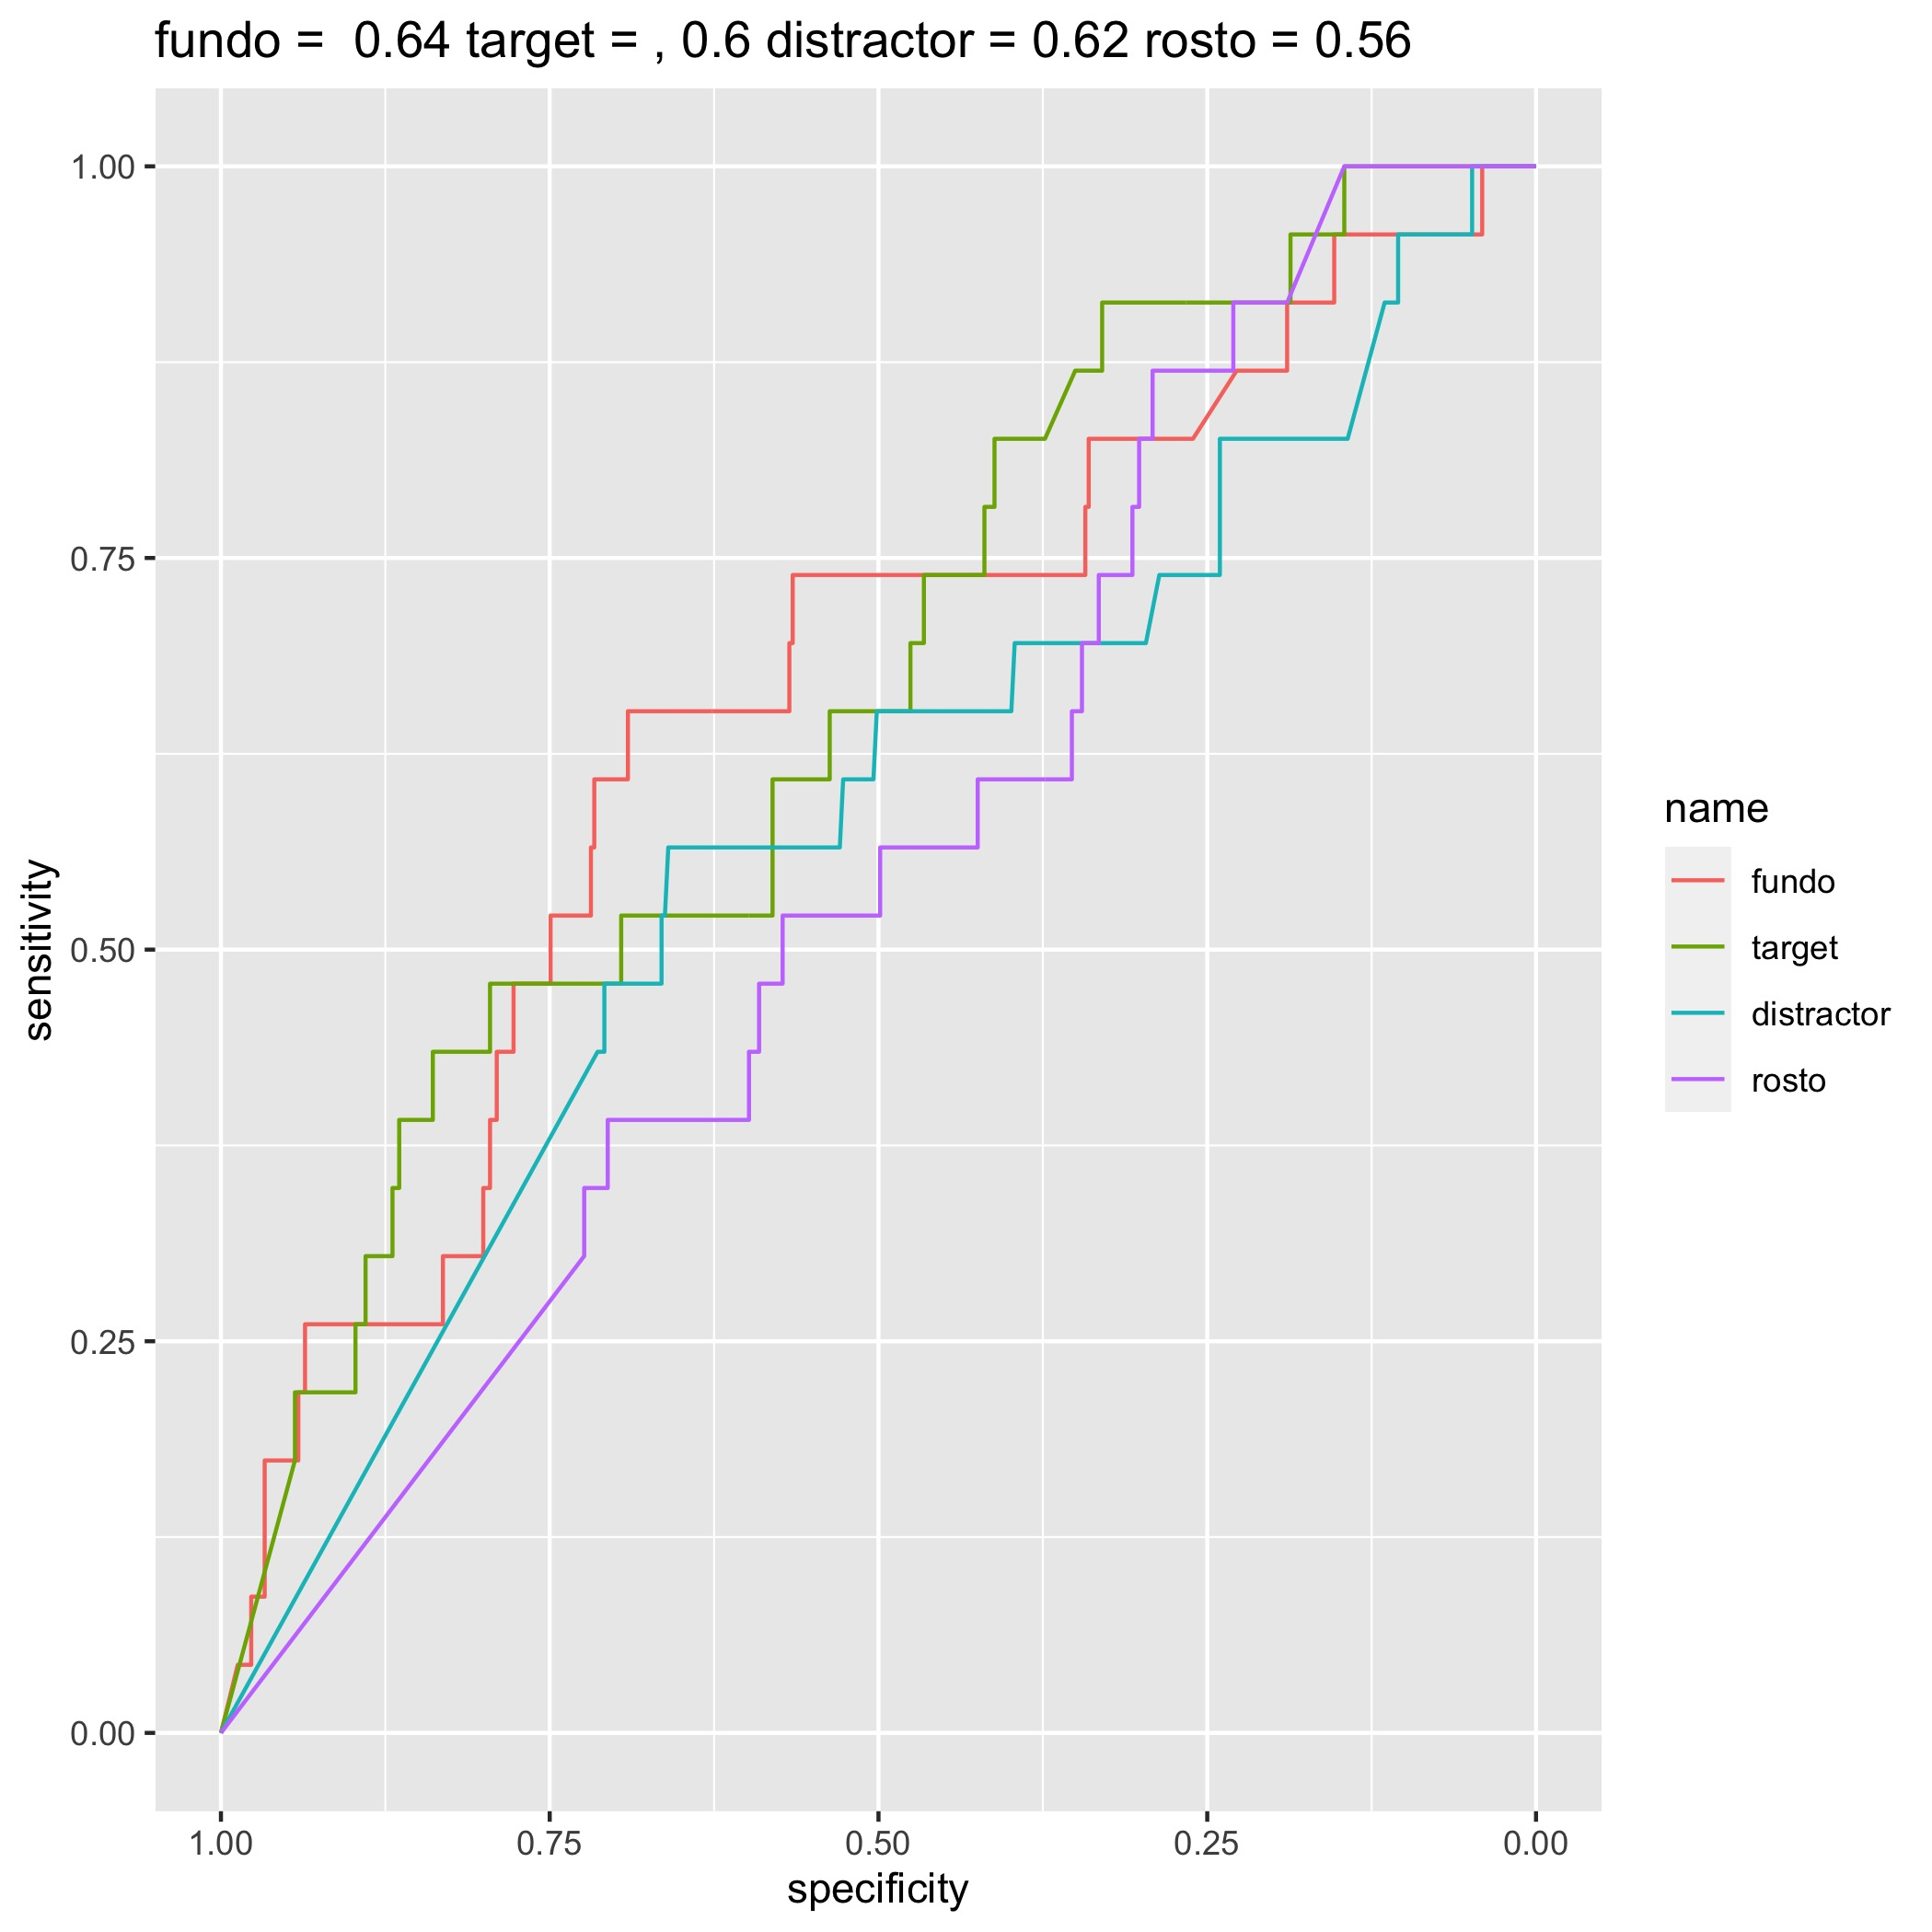
\includegraphics[scale=0.2]{./alternanciaNonMatched.jpg}}
  \centering
\end{figure}

\end{document}
